\documentclass[12pt, a4paper]{article}
\usepackage{multicol}
\usepackage{etoolbox}
\usepackage{relsize}
\usepackage{tikz}

\title{Rationality}
\author{Unknown}
\begin{document}
    \pagenumbering{gobble}
    \maketitle

    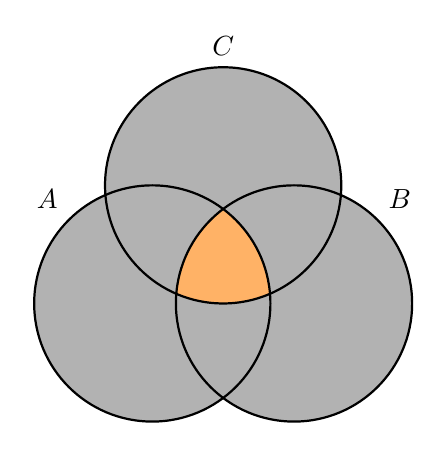
\begin{tikzpicture}[thick,
    set/.style = {circle,
        minimum size = 3cm,
        fill=black!30}]

% Set A
\node[set,label={135:$A$}] (A) at (0,0) {};

% Set B
\node[set,label={45:$B$}] (B) at (1.8,0) {};

% Set C
\node[set,label=$C$] (C) at (0.9,1.5) {};

% Intersection
\begin{scope}
    \clip (0,0) circle(1.5cm);
    \clip (1.8,0) circle(1.5cm);
    \clip (0.9,1.5) circle(1.5cm);
    \fill[orange!60](0,0) circle(1.5cm);
\end{scope}

% Circles outline
\draw (0,0) circle(1.5cm);
\draw (1.8,0) circle(1.5cm);
\draw (0.9,1.5) circle(1.5cm);
    \end{tikzpicture}

\end{document}
